% --------------------------------------------------------------------------- 
% Poster Template for Saikat Banerjee 
%
% Created with Brian Amberg's LaTeX Poster Template
% --------------------------------------------------------------------------- 
\documentclass[a0paper,portrait,debug]{baposter}


\usepackage{relsize}	% For \smaller
\usepackage{url}	% For \url
\usepackage{epstopdf}	% EPS files automatically to PDF to for pdflatex
\usepackage{multicol}
%\usepackage{amsmath}
\usepackage{amsmath,amssymb}
\usepackage{enumitem}
\graphicspath{{images/}}	% Root directory of the pictures 
\usepackage{helvet} %to use helvet font

\usepackage{charter}
%\usepackage[defaultsans]{droidsans}

\usepackage{siunitx}
\renewcommand{\familydefault}{\sfdefault} %set default font to sans-serif for entire document.

\usepackage{tikz}
\usetikzlibrary{shapes.geometric, arrows}
\tikzstyle{decision} = [rectangle, rounded corners, minimum width=3cm, minimum height=1cm, line width=1pt, text centered, align=flush center, draw=primary, fill=highlight!20]
\tikzstyle{origin} = [rectangle, rounded corners, minimum width=3cm, minimum height=1cm, line width=1pt, text centered, align=flush center, draw=subdue]%text=secondary]
\tikzstyle{highlight} = [rectangle, rounded corners, minimum width=3cm, minimum height=1cm, line width=1pt, text centered, align=flush center, draw=secondary, fill=important!30]%text=secondary]
\tikzstyle{textbox} = [rectangle, text centered, align=flush center] 
\tikzstyle{doubt} = [circle, line width=1pt, text centered, align=flush center, draw=secondary, fill=important!20]
\tikzstyle{arrow} = [thick,->,>=stealth]
\tikzstyle{line} = [thick, -]

\usepackage{varwidth}

\usepackage{bbding}

%------------------------------------------
\DeclareMathOperator{\logistic}{lf}
\DeclareMathOperator{\Var}{Var}
\DeclareMathOperator{\diag}{diag}
\DeclareMathOperator{\prob}{Pr}
\newcommand{\pvalue}{\mbox{$p\,$-value}}
\newcommand{\pvalues}{\mbox{$p\,$-values}}
\newcommand{\bs}{\boldsymbol}
\newcommand{\vx}{\mathbf{x}}
\newcommand{\vy}{\mathbf{y}}
\newcommand{\vz}{\mathbf{z}}
\newcommand{\vv}{\mathbf{v}}
\newcommand{\vX}{\mathbf{X}}
\newcommand{\vY}{\mathbf{Y}}
\newcommand{\vr}{\mathbf{r}}
\newcommand{\vtilde}{\tilde{\vv}}
\newcommand{\tss}[1]{\ensuremath{^{\text{\kern1pt\scriptsize #1}}}}
\newcommand{\N}{\mathcal{N}}


\newcommand{\eg}{{\it e.g.\ }}
\newcommand{\ie}{{\it i.e.\ }}
\newcommand{\etal}{{\it et al.\ }}
\newcommand{\avg}[1]{\left\langle #1 \right\rangle}
\newcommand{\abs}[1]{\left| #1 \right|}
\newcommand{\prth}[1]{\left( #1 \right)}
\newcommand{\brcs}[1]{\left\{ #1 \right\}}
\newcommand{\sqbr}[1]{\left[ #1 \right]}
\newcommand{\equn}{Eq}
\newcommand{\fign}{Fig}
\newcommand{\secn}{Sec.}
\newcommand{\figwidth}{1.0}
%-------------------------------------------

  


%%%%%%%%%%%%%%%%%%%%%%%%%
%%% Color Definitions %%%
%%%%%%%%%%%%%%%%%%%%%%%%%

\definecolor{gcmorange}{cmyk}{0,0.24,0.86,0.07}
%\definecolor{gcmorange}{cmyk}{0,0.43,0.95,0.01}
\definecolor{lightgray}{cmyk}{0,0.0,0.05,0.0}
\definecolor{lightblue}{cmyk}{0.06,0.03,0,0}
\definecolor{bluestone}{cmyk}{0.72,0.54,0,0.2}

\definecolor{primary}{RGB}{42,83,193} %% Cerulean blue #2A53C1
%\definecolor{primary}{cmyk}{0.782, 0.57, 0, 0.243}
\definecolor{secondary}{RGB}{240,60,63} %% Coral red #F03C3F
\definecolor{highlight}{RGB}{0, 180, 255} %% Blue bolt #00B4FF
\definecolor{light}{RGB}{255,255,243} %% White #FFFFF3
\definecolor{subdue}{RGB}{107,110,108} %% Grey #6B6E6C
\definecolor{black}{RGB}{43,40,40} %% #2B2828
\definecolor{hidden}{RGB}{160, 160, 160}
\definecolor{important}{RGB}{255, 142, 0} %% orange yellow #FF8E00
\definecolor{sub1}{RGB}{0, 125, 52} %% vivid green #007D34
\definecolor{sub2}{RGB}{255, 142, 0} %% strong violet #53377A

\definecolor{mpibpcgreen}{RGB}{190, 214, 52} %% orange yellow #FF8E00
\definecolor{mpibpcblue}{RGB}{26, 135, 162} %% vivid green #007D34
\definecolor{mpibpcmaroon}{RGB}{176, 88, 97} %% strong violet #53377A


\tikzstyle{highlight} = [rectangle, rounded corners, inner sep=1em, line width = 1pt, draw=secondary, fill=important!30]
\tikzstyle{highlightnosep} = [rectangle, rounded corners, inner sep=0.5em, line width = 1pt, draw=secondary, fill=important!30]
\tikzstyle{infoblock} = [rectangle, rounded corners, inner sep=1em, line width = 1pt, draw=primary, fill=highlight!20]
\tikzstyle{mathblock} = [rectangle, rounded corners, inner sep=1em, line width = 1pt, draw=primary, fill=highlight!20]

%%%%%%%%%%%%%%%%%%%%%%
%%% Poster Start %%%%%
%%%%%%%%%%%%%%%%%%%%%%
\begin{document}


%%%%reduce space between formulas
\setlength{\belowdisplayskip}{0pt} 
\setlength{\belowdisplayshortskip}{0pt} 
\setlength{\abovedisplayskip}{0pt} 
\setlength{\abovedisplayshortskip}{0pt}


\begin{poster}
{
% HINT: No newlines between options!
%
% SET LAYOUT PARAMETERS
%
	grid=false,
	columns=4,
	colspacing=1em,				% 1em is size of 'M' letter
	headerheight=15em, 				% header of poster
	eyecatcher=false,
	%
	% shades
	background=plain,
  	boxshade=plain,
	headershade=plain,  	
  	%
  	%shapes
	headershape=roundedright,		%boxtop
	textborder=rectangle,			%boxbottom
	linewidth=0.1ex,				%borderwidth
	headerfont=\rmfamily\scshape\bfseries\large,
	headerborder=open,
  	%
  	% colors
	bgColorOne=light, 
	borderColor=primary,
	headerColorOne=primary,
	headerColorTwo=primary,
	headerFontColor=white,
	boxColorOne=white,
	%
	%some positioning stuff
	boxpadding=0.5em,					%space between text and box [default 0.5em]
	boxheaderheight=2.3em				%height of box headers
}
{
% some graphics can be put on the left
}
%%% Title %%%
{
	{\color{primary}B-LORE}
}
%%% Sub-title
{
	{\color{primary}B}ayesian multiple {\color{primary}lo}gistic {\color{primary}re}gression for case-control GWAS%
}
%%% Authors %%
{		
	\underline{Saikat Banerjee}\textsuperscript{1}, Lingyao Zeng\textsuperscript{2}, Heribert Schunkert\textsuperscript{2} and Johannes S\"oding\textsuperscript{1}

}
{
	\textsuperscript{1} Max Planck Institute for Biophysical Chemistry, 37077 G\"ottingen, Germany\\
	\textsuperscript{2} German Heart Centre, 80636 Munich, Germany\\[0.5em]
        {\color{primary} \emph{saikat.banerjee@mpibpc.mpg.de, soeding@mpibpc.mpg.de}}
}
%%% Logo right of title %%%
{
\begin{tabular}{l l}
  \includegraphics[height=7em]{Max-Planck-Gesellschaft-no-txt.pdf} & \includegraphics[height=7em]{Print_Plotter_MPI-BPC_kurz-short_CMYK.eps} \\
\end{tabular}
}
{
	%\includegraphics[height=5em]{Print_Plotter_MPI-BPC_kurz-short_CMYK.eps}
}
%%%%%%%%%%%%%%%%%%%%%
%%% CONTENT BOXES %%%
%%%%%%%%%%%%%%%%%%%%%

%%%%%%%%%%%%%%%%%%%%%
%%% MOTIVATION %%%
%%%%%%%%%%%%%%%%%%%%%
\headerbox{1 Motivation}{name=motivation, column=0, row=0, span=4}{
  {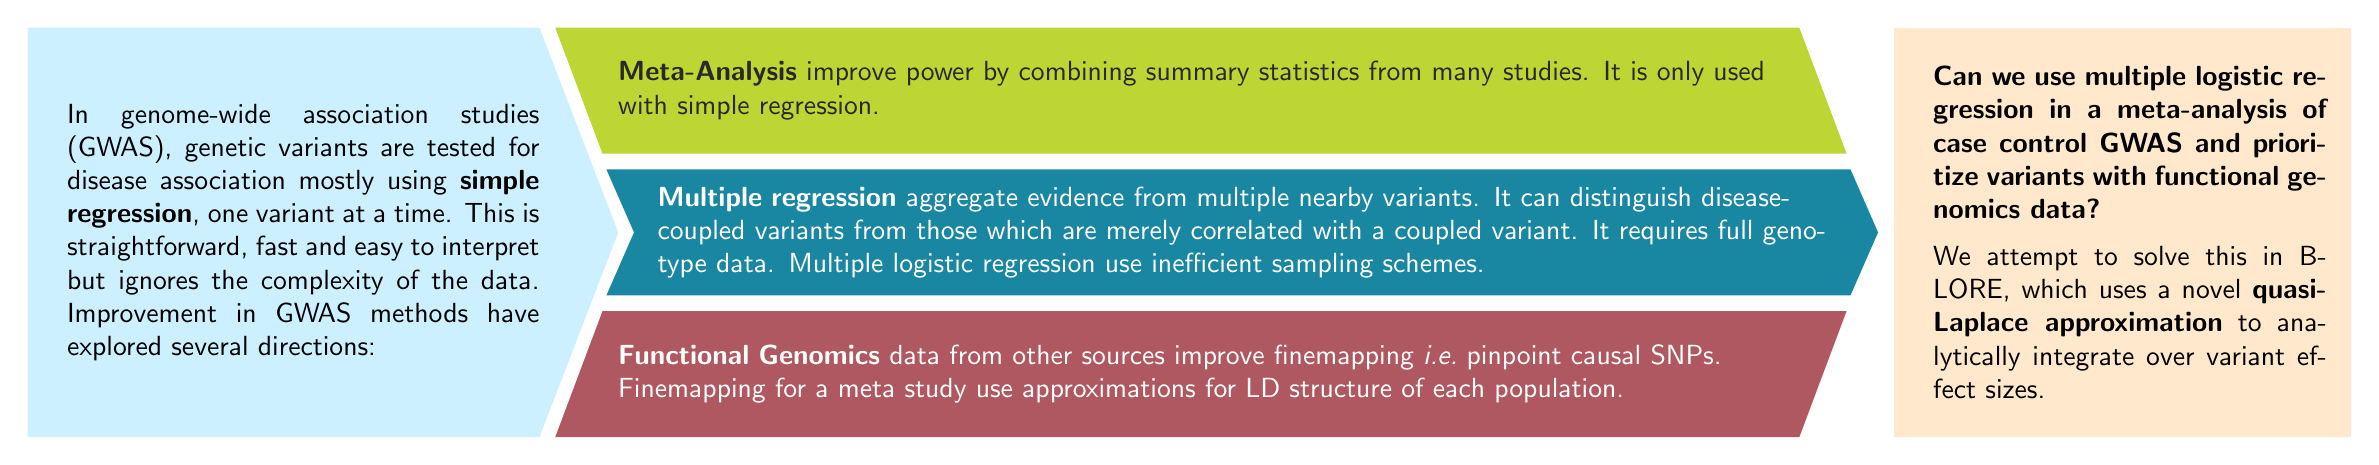
\begin{tikzpicture}
     \fill[fill = highlight!20] (0, 0) -- (6.5, 0) -- (7.5, 2.6) -- (6.5, 5.2) -- (0, 5.2) -- cycle;
     \node (simplereg) at (3.5, 2.6) [rectangle, align=justify, text width = 6cm, inner sep = 1em]
           {In genome-wide association studies (GWAS), genetic variants are tested for disease association mostly using \textbf{\textsc{simple regression}}, one variant at a time.
            This is straightforward, fast and easy to interpret but ignores the complexity of the data. Improvement in GWAS methods have explored several directions: };
     \fill[fill = mpibpcmaroon] (6.7, 0)    -- (22.5, 0.0) -- (23.1, 1.6) -- (7.3, 1.6)  -- cycle;
     \fill[fill = mpibpcblue] (7.35, 1.8) -- (23.15, 1.8) -- (23.5, 2.6) -- (23.15, 3.4) -- (7.35, 3.4) -- (7.7, 2.6) -- cycle;
     \fill[fill = mpibpcgreen] (7.3, 3.6)  -- (23.1, 3.6) -- (22.5, 5.2) -- (6.7, 5.2)  -- cycle;
     \node (improve1) at (15.0, 4.4) [rectangle, align=left, text width = 15cm, inner sep = 0em, color = black]
           {\textbf{\textsc{Meta-Analysis}} improve power by combining summary statistics from many studies.
             It is only used with simple regression.
            };
     \node (improve2) at (15.5, 2.6) [rectangle, align=left, text width = 15cm, inner sep = 0em, color = white]
           {\textbf{\textsc{Multiple regression}} aggregate evidence from multiple nearby variants.
            It can distinguish disease-coupled variants from those which are merely correlated with a coupled variant. 
            It requires full genotype data. Multiple logistic regression use inefficient sampling schemes.};
     \node (improve3) at (15.0, 0.8) [rectangle, align=left, text width = 15cm, inner sep = 0em, color = white]
           {\textbf{\textsc{Functional Genomics}} data from other sources improve finemapping \ie pinpoint causal SNPs.
            Finemapping for a meta study use approximations for LD structure of each population.};%
     \fill [fill = important!20, inner sep = 0em] (23.7, 0) -- (29.5, 0) -- (29.5, 5.2) -- (23.7, 5.2) -- cycle;
     \node (blore) at (26.7, 2.6)%
           [rectangle, align=justify, text width = 5cm, inner sep = 0em]
           {\textbf{Can we use multiple logistic regression in a meta-analysis of case control GWAS and prioritize variants with functional genomics data?}
            \\[0.5em] We attempt to solve this in B-LORE, which uses a novel \textbf{quasi-Laplace approximation} to analytically integrate over variant effect sizes.};
   \end{tikzpicture}
  }%
}

%%%%%%%%%%%%%%%%%%%%%
%%% METHODS %%%
%%%%%%%%%%%%%%%%%%%%%
\headerbox{2 Model and Priors}{name=model, column=0, row=1, span=2, below=motivation}{

  Probability of $n$\tss{th} individual with genotype $\vx_n$ to be diseased:
  \begin{multicols}{2}
    {\begin{center}
      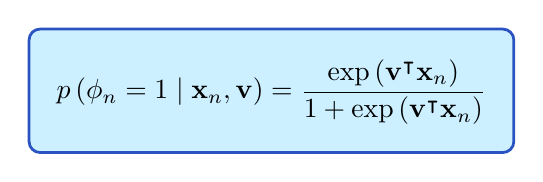
\begin{tikzpicture}
        \node (a) at (0,0) [mathblock] {
          \begin{varwidth}{\linewidth}
          \begin{equation*}
            p\prth{\phi_n = 1 \mid \vx_n, \vv} = \frac{ \exp\prth{\vv^{\intercal}\vx_n} }{ 1 + \exp\prth{\vv^{\intercal}\vx_n} }
          \end{equation*}
          \end{varwidth}
        };
      \end{tikzpicture}
    \end{center}}
    {\begin{center} 
      \includegraphics[width=0.4\textwidth]{logistic_function_02.pdf}
    \end{center}}
  \end{multicols}
  {\vspace{-2em}}%\color{primary}\noindent\rule{0.4\linewidth}{0.4pt}}\\[0.5em]
  Prior on effect sizes given hyperparameters $\bs\theta$ ($\pi, \mu, \sigma, \sigma_\text{bg}$),
  {\vspace{-1em}}%\color{primary}\noindent\rule{0.4\linewidth}{0.4pt}}\\[0.5em]
  \begin{multicols}{2}
    {$\!
    \begin{aligned}
      & p\prth{v_i \mid \bs\theta} \nonumber\\ &=  
                                    {\color{secondary}\overbrace{\pi_i\,\N\prth{v_i \mid \mu, \sigma^2}}^{\text{Causal}}} +
                                    {\color{primary}\overbrace{\prth{1 - \pi_i} \N\prth{v_i \mid 0, \sigma^2_\text{bg}}}^{\text{Non-causal}}} \nonumber \\[0.75em]
                                 &= \sum_{z_i = 0, 1} {\color{secondary} \pi_i^{z_i}} {\color{primary}\prth{1 - \pi_i}^{\prth{1 - z_i}}} \nonumber \\[-1em]
                                 & \qquad \qquad \qquad \times \N\prth{ v_i \mid \bs\mu_{\vz, i}, \diag(\bs\sigma^2_{\vz, i}) } \nonumber
      \label{eq:effectsize-prior}
    \end{aligned}
    $\\[1em]
    $\mu_{\vz,i} = z_i \mu$ \\[0.5em]
    $\sigma^2_{\vz,i} = \sigma^2_\text{bg} + z_i \prth{\sigma^2 - \sigma^2_\text{bg}}$ \\[0.5em]
    {$\displaystyle
      \pi_i = \frac{1}{1 + \exp\prth{ - \bs\xi_i^{\intercal} \bs\beta_\pi} }
    $}\\[1em]
    {$z_i \in \{0, 1\} \Rightarrow$ Indicator variable of causality} \\[0.5em]
    {$\bs\xi_i \Rightarrow$ vector of local genomic features}
    }%
    {\begin{center}
      \includegraphics[width=0.43\textwidth]{bayesian_logistic_regression_01.pdf} \\[1em]
      %{$z_i \in \{0, 1\} \Rightarrow$ Indicator variable of causality} \\[0.5em]
      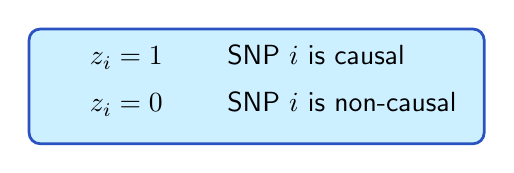
\begin{tikzpicture}
        \node (a) at (0,0) [infoblock] {
            \begin{varwidth}{\linewidth}
            \begin{itemize}[leftmargin=1.2em, label={\color{primary}\tiny\DiamondSolid}]
              \setlength\itemsep{0.1em}
              \item $z_i = 1$ \qquad SNP $i$ is causal
              \item $z_i = 0$ \qquad SNP $i$ is non-causal
            \end{itemize}
            \end{varwidth}
        };
      \end{tikzpicture}
    \end{center}}
  \end{multicols}
}

\headerbox{3 Optimization}{name=optim, column=2, span=2, below=motivation, bottomaligned=model}{

  \emph{Evidence approximation}: maximizing the marginal likelihood\\[-0.5em]
  \begin{equation*}
    mL(\bs\theta) = p \prth{ \bs\phi \mid \vx, \bs\theta }
                  = \sum_{\vz} {\color{sub1} p\prth{ \vz \mid \bs\theta }}
                     \int {\color{sub2} p \prth{ \bs\phi \mid \vx, \vv }}\,
                          {\color{sub1} \mathcal{N}\prth{ \vv \mid \bs\mu_\vz, \diag\prth{\bs\sigma^2_\vz} }}
                          d\vv
                 \rightarrow \max
  \end{equation*}

  \vspace{0.75em}
  {\textbf{Quasi-Laplace approximation}:}
  \begin{equation*}
    {\color{sub2} p\prth{ \bs\phi \mid \vx, \vv }}\, {\color{sub1} \mathcal{N}\prth{ \vv \mid \bs\mu_\vz, \diag\prth{\bs\sigma^2_\vz} }} =
       {\color{black} \underbrace{ {\color{sub2} p\prth{ \bs\phi \mid \vx, \vv }}\, {\color{black} \mathcal{N}\prth{\vv \mid \tilde{\bs\mu}, \diag\prth{\tilde{\bs\sigma}^{2}} }} }_{
                       \displaystyle \propto \mathcal{N} \prth{ \mathbf{v} \mid \tilde{\vv}, \tilde{\bs\Lambda}^{-1} }}
       }
      \times \frac{{\color{sub1}\mathcal{N}\prth{ \vv \mid \bs\mu_\vz, \diag\prth{\bs\sigma^2_\vz} }}}{\color{black} \mathcal{N}\prth{\vv \mid \tilde{\bs\mu}, \diag\prth{\tilde{\bs\sigma}^{2}} }}
  \end{equation*}

  \vspace{1em}
  The optimization can be done over multiple studies,
  \begin{equation*}
    mL(\bs\theta) = p \left( \bs\phi \mid \vx_1, \vx_2, \ldots , \vx_S, \bs\theta \right)
                  = \int p \left( \bs\phi \mid \vx_1, \vx_2, \ldots , \vx_S, \vv \right) p \left( \vv \mid \bs\theta \right) d\vv \rightarrow \max
  \end{equation*}

  \vspace{0.5em}
  assuming that the quasi-Laplace approximation holds for each individual study
  {\color{primary}
  \begin{equation*}
    \prod_{s=1}^{S} \left[ p \left( \bs\phi \mid \vx_s, \vv \right) \mathcal{N} \left( \mathbf{v} \mid \tilde{\bs\mu}_{\vz,s}, \diag(\tilde{\bs\sigma}_{\vz,s}^2) \right) \right]
        \propto \prod_{s=1}^{S} \mathcal{N} \left( \vv \mid \tilde{\vv}_s, \tilde{\bs\Lambda}_s^{-1} \right)
        = \mathcal{N} \left( \vv \mid \tilde{\vv}, \tilde{\bs\Lambda}^{-1} \right)
  \end{equation*}
  }
  where $\displaystyle \tilde{\bs\Lambda} = \sum_{s=1}^{S} \tilde{\bs\Lambda}_s$ and $\displaystyle \tilde{\vv} = \tilde{\bs\Lambda}^{-1} \sum_{s=1}^{S} \tilde{\bs\Lambda}_s \tilde{\vv}_s$.
  {\begin{center}
    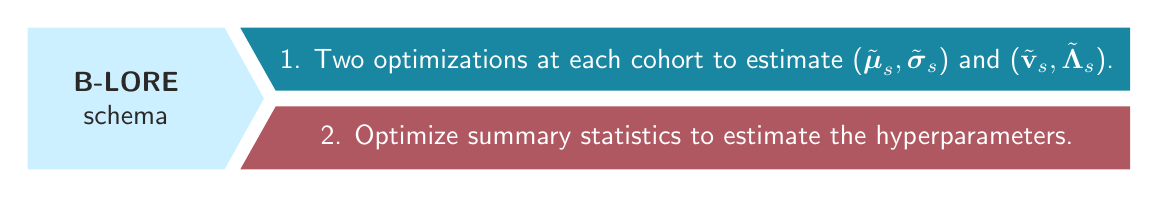
\begin{tikzpicture}
      \fill[fill = highlight!20] (0, 0) -- (2.5, 0) -- (3, 0.9) -- (2.5, 1.8) -- (0, 1.8) -- cycle;
      \fill[fill = mpibpcmaroon] (2.7, 0) -- (14, 0) -- (14, 0.8) -- (3.15, 0.8) -- cycle;
      \fill[fill = mpibpcblue]   (3.15, 1) -- (14, 1) -- (14, 1.8) -- (2.7, 1.8) -- cycle;
      %\fill[fill = mpibpcmaroon!80] (5, 0) -- (14, 0) -- (14, 0.8) -- (5, 0.8) -- cycle;
      %\fill[fill = mpibpcblue!80]   (5, 1) -- (14, 1) -- (14, 1.8) -- (5, 1.8) -- cycle;
      \node at (1.25, 0.9) [rectangle, align=center, text width = 2cm, inner sep = 0em, color=black] {\textbf{B-LORE} schema};
      \node at (8.5, 1.4) [rectangle, align=center, inner sep = 0em, color=white]
                          {1. Two optimizations at each cohort to estimate  ($\tilde{\bs\mu}_{s}, \tilde{\bs\sigma}_{s}$) and ($\tilde{\vv}_s, \tilde{\bs\Lambda}_s$).};
      \node at (8.5, 0.4) [rectangle, align=justify, inner sep = 0em, color=white]
                          {2. Optimize summary statistics to estimate the hyperparameters.};
    \end{tikzpicture}
  \end{center}}

}

\headerbox{4 Inference}{name=infer, column=3, span=1, below=optim}{
  {\color{primary}\emph{Prediction of causality of each locus}.}\\[0.5em]
  The probability for a locus to be causally associated with the disease is%= 1 -- probability of {\scshape not} containing a single causal SNP.
  {\begin{center} \vskip-0.25em
    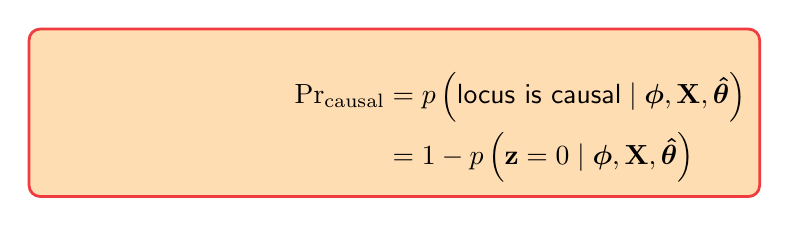
\begin{tikzpicture}
      \node (a) at (0,0) [highlightnosep] {
          \begin{varwidth}{\linewidth}
            \begin{align*}
              \prob_{\mathrm{causal}} &= p\prth{\text{locus is causal} \mid \bs\phi, \vX, \bs{\hat\theta}} \\
                                      &= 1 - p\prth{\vz = 0 \mid \bs\phi, \vX, \bs{\hat\theta}}
            \end{align*}
          \end{varwidth}
      };
    \end{tikzpicture}
  \end{center}}

  {\color{primary}\emph{Statistical finemapping of causal variants}.}\\[0.5em]
  The posterior probability for SNP $i$ to be causal is 
  {\begin{center} \vskip-0.5em
    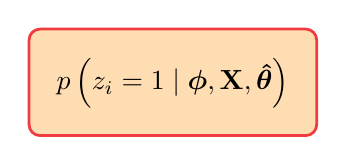
\begin{tikzpicture}
      \node (a) at (0,0) [highlight] {
          \begin{varwidth}{\linewidth}
            \begin{equation*}
              p\prth{z_i = 1 \mid \bs\phi, \vX, \bs{\hat\theta}}
            \end{equation*}
          \end{varwidth}
      };
    \end{tikzpicture}
  \end{center}}
}

%%%%%%%%%%%%%%%%%%%%%%%%%%%%%%%%%%%
%%%% GERMIFS CAD %%%
%%%%%%%%%%%%%%%%%%%%%%%%%%%%%%%%%%%
\headerbox{5 Application on Coronary Artery Disease}{name=realcad, column=0, span=3, below=model}{
\newdimen\myfigheight
\setlength{\myfigheight}{8cm}

  \begin{center}
    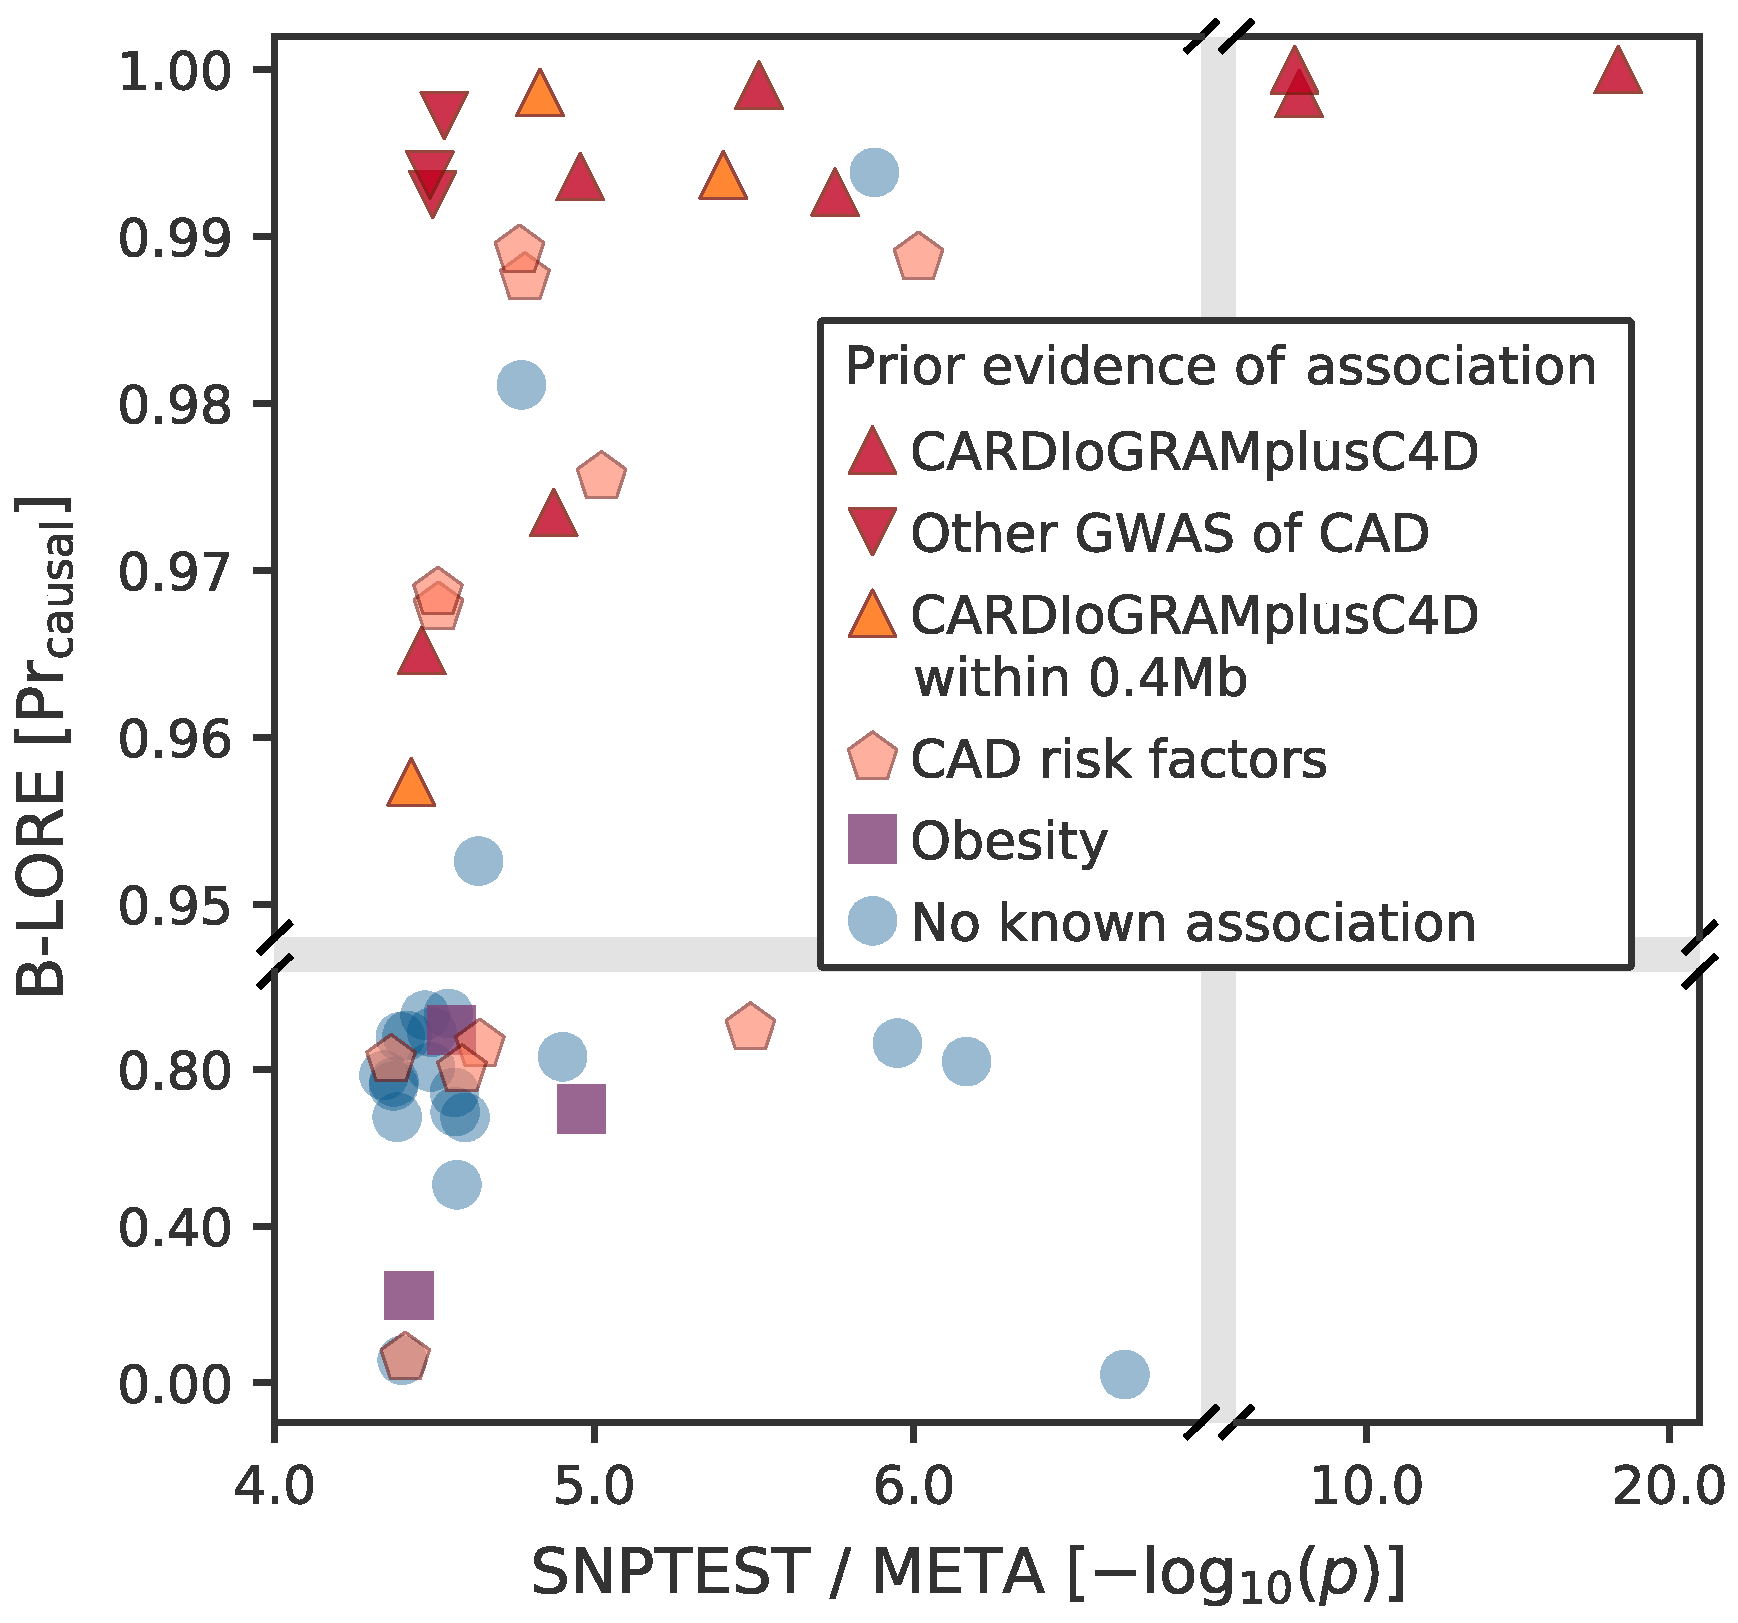
\includegraphics[height=\myfigheight, keepaspectratio]{loci_classification.pdf}
    \includegraphics[height=\myfigheight, keepaspectratio]{Locus_018.pdf}
    \includegraphics[height=\myfigheight, keepaspectratio]{Locus_013.pdf}
  \end{center}
Meta-analysis of 5 cohorts (Germal Myocardial Infarction Family Study, GerMIFS I-V) with a total of 6234 cases and 6848 controls from white European ancestry. 
We pre-selected the top 50 loci with SNPTEST / META, and applied B-LORE, using 112 functional genomics features for each SNP from DNase-seq data of the ENCODE project.
}


%%%%%%%%%%%%%%%%%%%%%%%%%%%%%%%%%%e
%%%% SIMULATION RESULTS %%%
%%%%%%%%%%%%%%%%%%%%%%%%%%%%%%%%%%%
\headerbox{6 Meta-analyses with real genotype and simulated phenotype }{name=simures, column=0, span=3, below=realcad}{

  {We selected 200 loci each with 200 SNPs from GerMIFS. We used 112 functional genomics features.
  We randomly selected 3 features as significant and simulated binary phenotype for $\sim$ 13000 patients.
  Each simulation had 100 causal loci and $\sim$ 450 causal SNPs with a total heritability of 0.25.}

\begin{multicols}{4}
  \includegraphics[width=0.23\textwidth]{simu_locus_scatter_nold_nofeat.pdf}
  \includegraphics[width=0.23\textwidth]{simu_locus_precision_recall_nold.pdf}
  \includegraphics[width=0.23\textwidth]{simu_finemap_recall_nold_30SNPs.pdf}
  \includegraphics[width=0.23\textwidth]{simu_finemap_precision_recall_nold.pdf}
\end{multicols}
}

%%%%%%%%%%%%%%%%%%%%%%%%%%%%%%%%%%
%%%% REFERENCES %%%
%%%%%%%%%%%%%%%%%%%%%%%%%%%%%%%%%%
\headerbox{7 References}{name=biblio, column=3, span=1, below=realcad, below=infer}{
 {\raggedright
  \footnotesize
 \begin{enumerate}[leftmargin=1.5em]
   \item Banerjee \etal bioRxiv 2017, doi:10.1101/198911
   \item Servin \etal PLOS Genet 2007, doi:10.1371/ journal.pgen.0030114
   \item Guan \etal Ann Appl Stat 2011, doi:10.1214/ 11-AOAS455
   \item Schunkert \etal, Nat Genet 2011, doi:10.1038/ ng.784
   \item CARDIoGRAMplusC4D Nat Genet 2015, doi:10.1038/ng.3396
 \end{enumerate}
 }
}

\headerbox{8 Acknowledgement}{name=thanks, column=3, span=1, below=biblio}{

  \footnotesize
  We thank Prof. Dr. Jeanette Erdmann and all members of the S\"oding lab for helpful suggestions and discussions.
  This work was supported by the German Federal Ministry of Education and Research (BMBF) within the framework of
  the e:Med research and funding concept (grant 01ZX1313A-2014).

  \begin{minipage}{\textwidth}
    \centering
    \raisebox{-0.5\height}{\includegraphics[height=75px]{BMBF.eps}}
    %\hspace*{.2in}
    \raisebox{-0.5\height}{\includegraphics[height=37px]{emed_logo.png}}
  \end{minipage}
}

\end{poster}
\end{document}
